\chapter{Methods}

\section{Microscope setup}

\begin{figure}
	\centering
	\includegraphics[width=\linewidth]{microscope layout.pdf}
	\caption{
		Schematic overview of the Tegenfeldt microscope. The sample is located in a microscope housing on the bottom right (outside this figure). FC1 and FC2 are filter cube housings. Half-wave and quarter-wave plates are denoted $ \lambda/2 $ and $ \lambda/4 $, respectively. Dashed lines represent the light path, except those that go to the TCSPC (those are digital connections). The waveplates in the pSTED module were not in the original setup, and were added by us. See text for more details.
	}
	\label{fig:layout}
\end{figure}

The Tegenfeldt microscope is a confocal fluorescence microscope constructed by Abberior Instruments GmbH (Germany). It features two excitation lasers (at 561~nm and 640~nm) and one depletion laser at 775~nm for two-channel confocal or STED microscopy. It also contains a time-correlated single photon counter (TCSPC) for fluorescence lifetime imaging microscopy (FLIM) and a highly sensitive photomultiplier tube (PMT). Refer to \autoref{fig:layout} for the layout of these optical elements. Samples are located inside an inverted Nikon microscope body (Ti-E, not shown in the figure) equipped with a piezo stage (M-687 PILine XY-stage system and P-736 PInano (Physik Instrumente) Z Microscope Scanner), a 60x, 1.4~NA oil immersion objective (Nikon Plan Apo) and a QUADScan beam scanner (Cambridge Technology).


In this section, I will address all laser lines as well as the detection module in detail, with a focus on characterising the light polarisation at different points in the microscope.

\paragraph{The excitation lasers.} This fast-switching 561~nm laser is initially horizontally polarised, but the polarisation can be tuned by three waveplates in its path. The last one, a quarter-wave plate, is fixed in its rotation angle. In the standard mode of operation, excitation laser light should be circularly polarised to minimise resolution reduction due to lens distortion etc. \cite{Harke2008}. In that mode, the (fast or slow) axis of the first quarter-wave plate should be aligned with the laser, such that it does not affect polarisation and the half-wave plate should be set such that it rotates the (linearly polarised) light to \ang{45} with respect to the second quarter-wave plate. See \todo{table} for the polarisation characteristics in the calibration provided by Abberior. \todo{mention in words that it's very good} 

The 640 nm laser does not have fast-switching built in, so instead the light is fed into the microscope through a polarisation-polarisation optical fibre by an acousto-optical modulator (AOM). The AOM is a crystal in the beam path, in which sound waves can be generated by a piezo element. The ray is deflected by an angle that depends on the frequency of these waves, such that the laser beam can quickly be aligned into or away from the fibre aperture. The rest of the beam path is very similar to the 561 module, but the calibration of the waveplates in this pathway are not as accurate. Refer to \todo{table}.

\paragraph{The STED module.} The depletion laser travels through an entirely different set of optics than the excitation lasers to generate a donut beam. First, it travels through a half-wave plate that aligns the polarisation to the SLM (spatial light modulator). The SLM adds an arbitrary spatially patterned phase delay to the light falling on it, but only if light is polarised along its active axis. It will not alter the phase of the orthogonally polarised component. Using the proper phase delay patterns, one can create any (diffraction-limited) image in the sample plane. In our case, that would be a donut shape. Then -- and I am ignoring the pSTED module for now -- the light travels through a half-wave plate to ensure circular polarisation in the sample plane, just like the excitation lasers. This is done to ensure that the depletion efficiency does not depend on sample orientation and to avoid polarisation-dependent PSF distortion by lenses and other optics. 

\paragraph{The detection module.} The main detectors of the microscope are a set of avalanche photodiodes (APDs), but there is also a highly sensitive photomultiplier tube (PMT) right after the QWP on the microscope end. The PMT is usually used to measure the point spread functions of the lasers and to align them. In normal operation, the light travels on to the detection waveplates, then through a pinhole wheel, passes filters and dichroics in the filter cube housings, and is finally reflected onto the APDs. The wheel contains pinholes of different sizes, which allows for choosing the trade-off between light collection and $ z $ resolution. Different filter cubes are available with various notch filters, dichroic mirrors, and/or a polarising beam splitter (PBS).

The APDs show a slight polarisation sensitivity, of about 10\% of the maximum sensitivity (see \autoref{fig:apd pol sensitivity}). I measured this by exciting Tetraspec beads with the 561 laser set to circular excitation, such that the emission light is non-polarised. Then I put a linear polariser on  \todo{This actually seems to be on the order of the 561 circularity error! Analyse that data.}

We did have some problems with the waveplates in the detection module. They can be controlled through Abberior's software suite (Imspector), but it is not clear if they are set up correctly. The calibration is based on a control angle that I will call $ \theta $. It would be possible for this setup to rotate polarised light of any orientation, since
\begin{equation}
	S_\hwp(\theta/2) S_\qwp(0) S_\qwp(0) = \mqty(\cos\theta & -\sin\theta \\ \sin\theta & \cos\theta ),
\end{equation}
which is simply the rotation matrix $ R(\theta) $. The exact position of the quarter-wave plates does not matter, but it is important that they are aligned with each other. If the waveplates are at a different angle $ \phi $, then this set of waveplates rotates the polarisation by an angle $ (\theta-2\phi) $ instead. It is worth noting that the calibration provided by Abberior does something completely different, that we don't yet understand, so I developed a new calibration.

First, I had to figure what angle to set the second quarter-wave plate to in order to align it to the first one. I did this by placing a polariser in the sample holder (P1) and illuminating it with the top lamp, such that the light incident on the first quarter-wave plate was linearly polarised. Then I placed another polariser (P2) after the waveplates that I rotated to assess the linearity of the polarisation there. Aligning the quarter-waveplates with each other simply involved maximising the linearity. 

Second, I assessed both Abberior's and my calibration. As presented in \autoref{fig:detection waveplate calibrations}, my calibration works really well. \todo{Mention the problem and how we might fix it.}

\begin{figure}
	\centering
	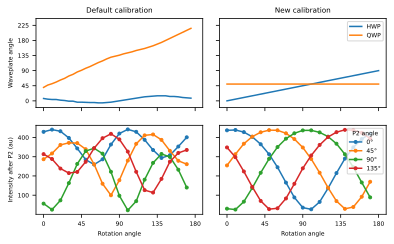
\includegraphics{detection_waveplate_calibrations.pdf}
	\caption{\todo{text}}
	\label{fig:detection waveplate calibrations}
\end{figure}

\todo{Mention the pol cube results.}

\section{Data analysis of conventional polarisation images}

\section{Polarisation-resolved STED microscopy (pSTED)}

\section{Samples used in this thesis}
